\documentclass[11pt,letterpaper]{refart}

\usepackage{gitinfo2}
\usepackage{amsmath,mathtools}

\usepackage{hyperref}
\usepackage{cleveref}
\usepackage{caption}
\usepackage{subcaption}

\usepackage{microtype}
\usepackage[T1]{fontenc}

\usepackage{graphicx}
\usepackage{xcolor}
\usepackage{framed}
\usepackage{booktabs}
\usepackage{siunitx}  % Better kerning

\usepackage{tikz}
\tikzset{
    boximg/.style={remember picture,
                   ultra thick,
                   inner sep=0pt,
                   outer sep=0pt}
}

\usepackage{listings}
\lstset{
	basicstyle=\ttfamily\footnotesize,
	breaklines=true,
	postbreak=\mbox{\textcolor{red}{$\hookrightarrow$}\space},
	frame=single,
	columns=flexible
}

\def\itwoc{I{$\scriptstyle^2$}C\ }
\newcommand\symbolwithin[2]{%
{\mathmakebox[\widthof{\ensuremath{{}#2{}}}][c]{{#1}}}}

\title{DCB Design Verification Measurements}
\author{University of Maryland LHCb group}

\begin{document}
\maketitle
\hfill\small{\texttt{Rev:~\gitRel~(\gitAbbrevHash)}}
\tableofcontents


\section{Transient current}
We used a Gauss probe connected to an oscilloscope to measure current.
The probe was warped around the cable which was connected to the positive end of
the \SI{1.5}{\volt} PSU.

All the measurements below assume a conversion factor of \SI{1}{\ampere/\volt}.
All measurements are made on DCB pilot S/N 007.

\subsection{Power on}
\begin{figure}[ht]
    \centering
    \begin{subfigure}{0.8\linewidth}
    \begin{tikzpicture}[boximg]
        \node [anchor=south west] (main) {
            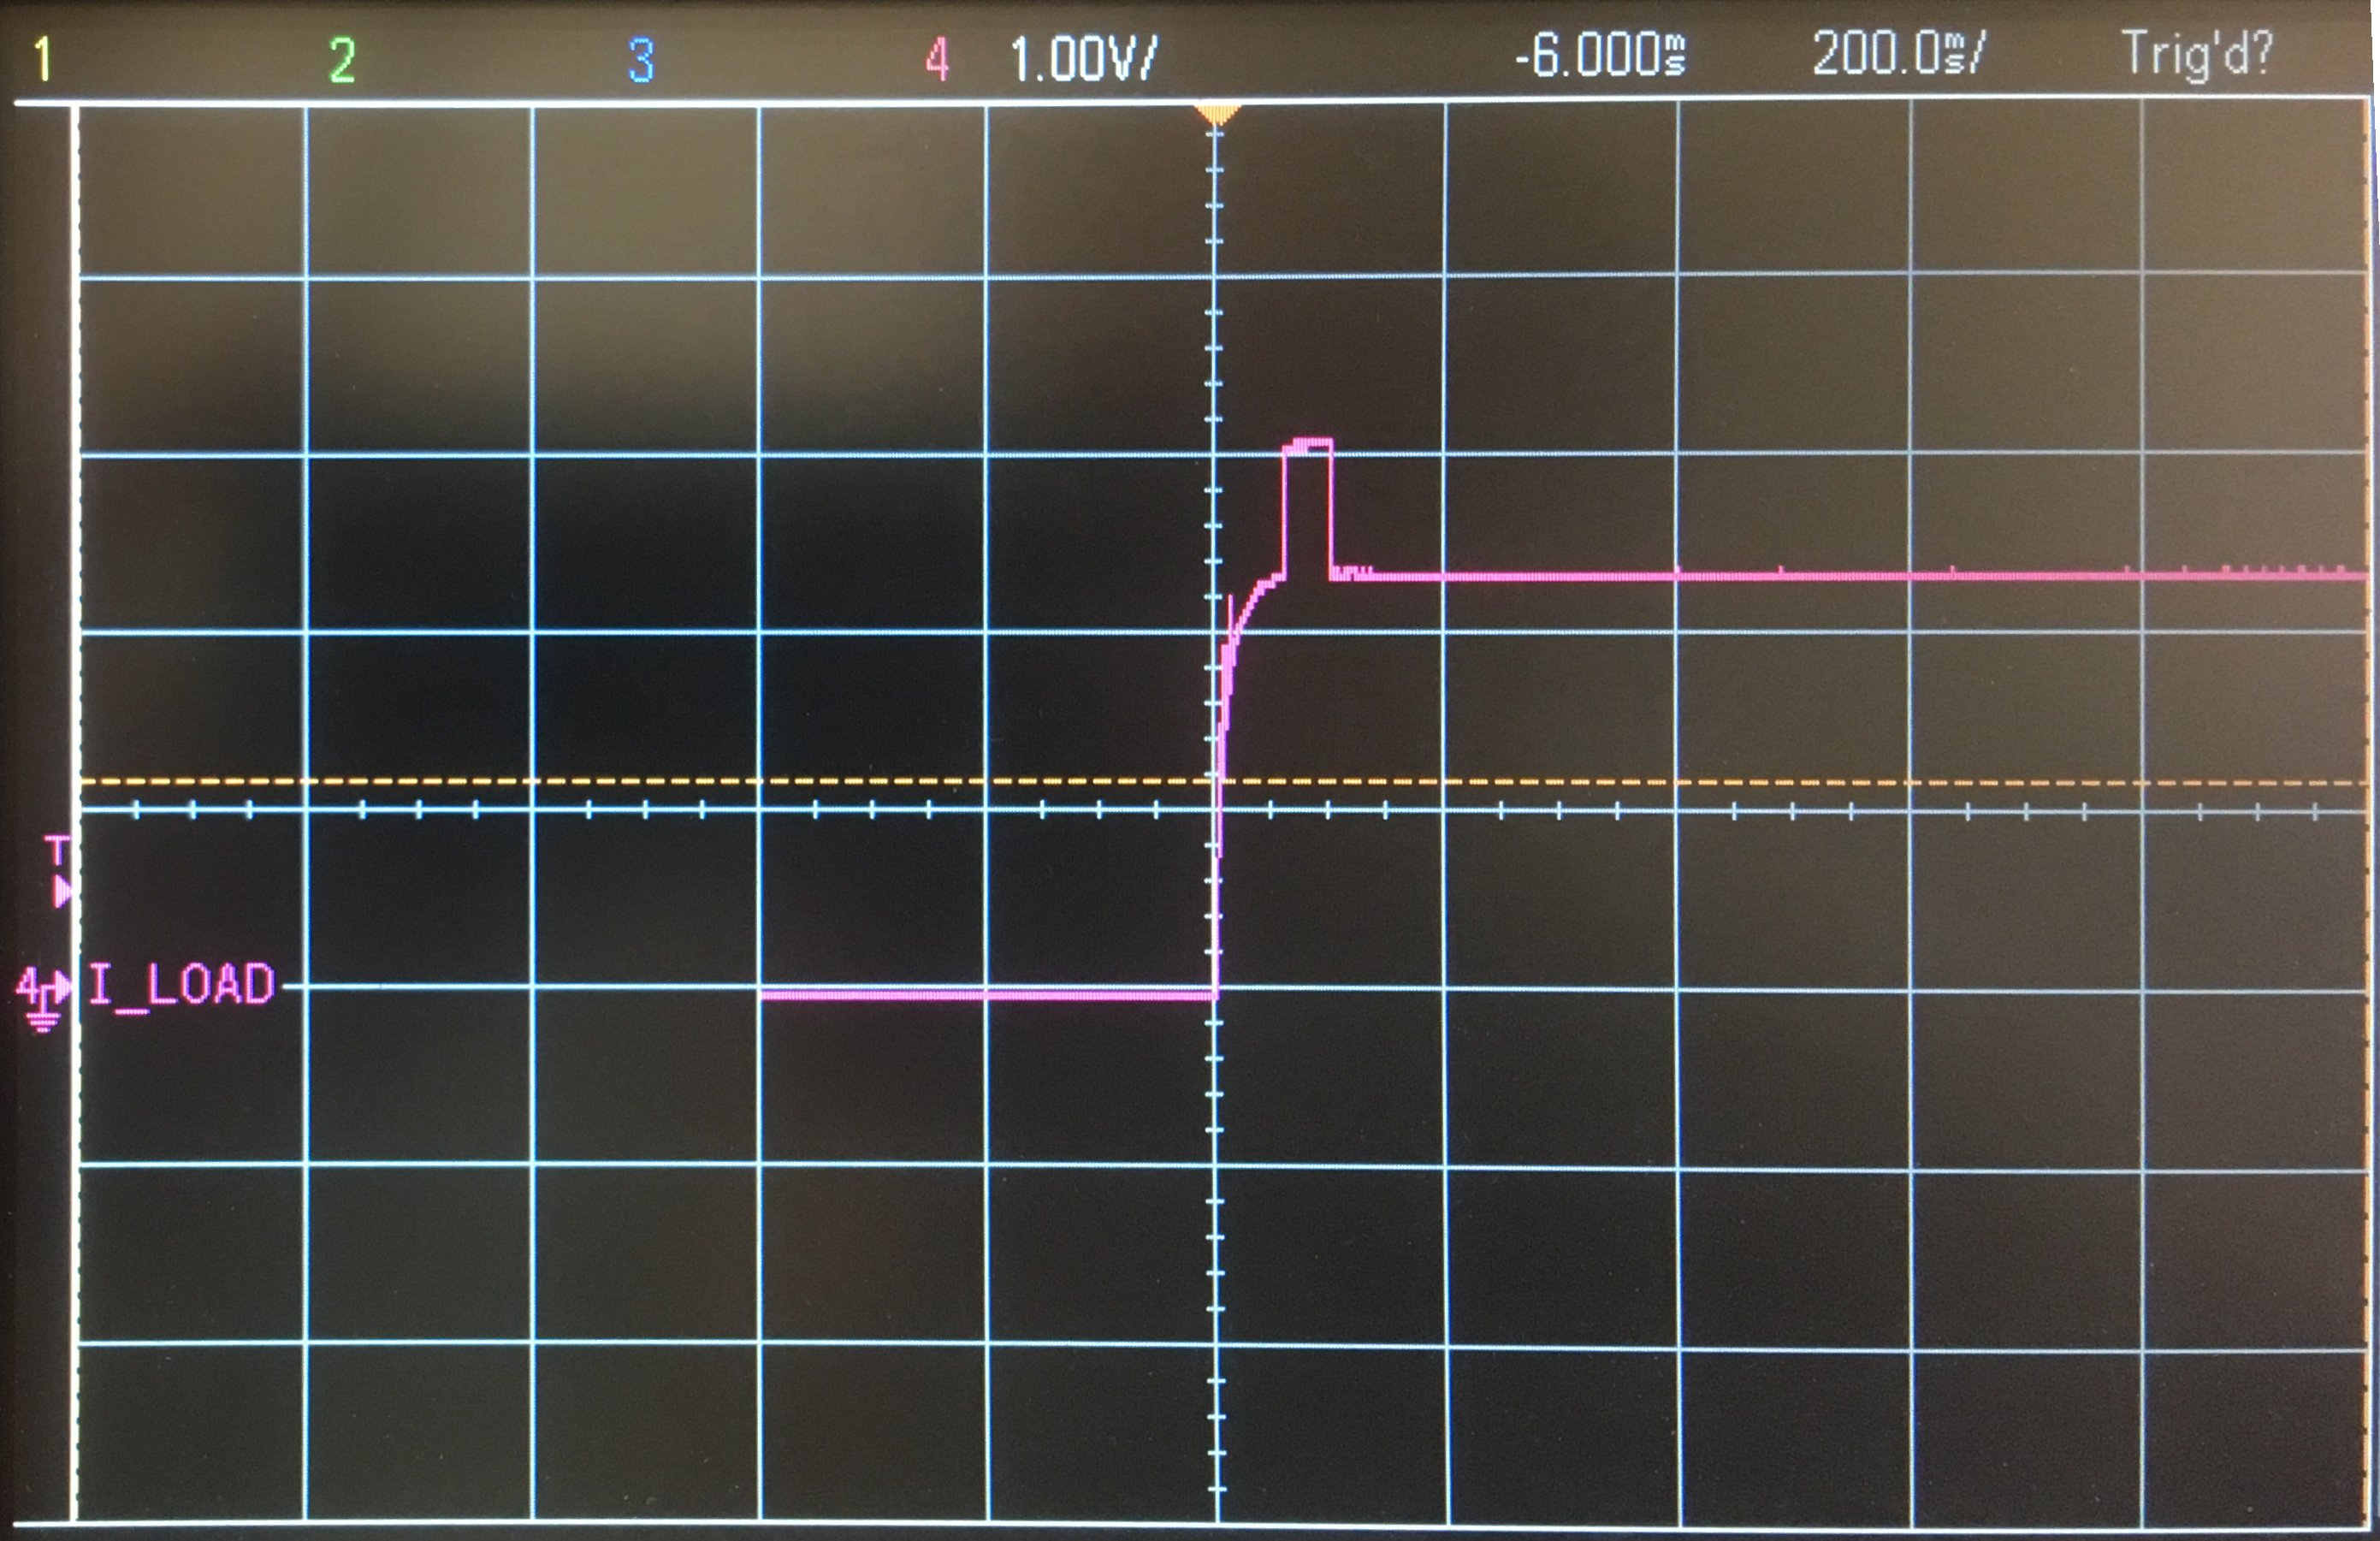
\includegraphics[width=\linewidth]
            {./res/current_transient/power_on.jpg}
        };
        \begin{scope}[x=(main.south east),y=(main.north west)]
            \node[draw,orange,minimum height=5em, minimum width=2em] (zoombox1)
            at (0.5,0.5) {};
        \end{scope}
    \end{tikzpicture}
    \caption{}
    \end{subfigure} \\[0.5\baselineskip]
    \begin{subfigure}{0.5\linewidth}
    \begin{tikzpicture}[boximg, orange]
        \node  (zoom1) {
            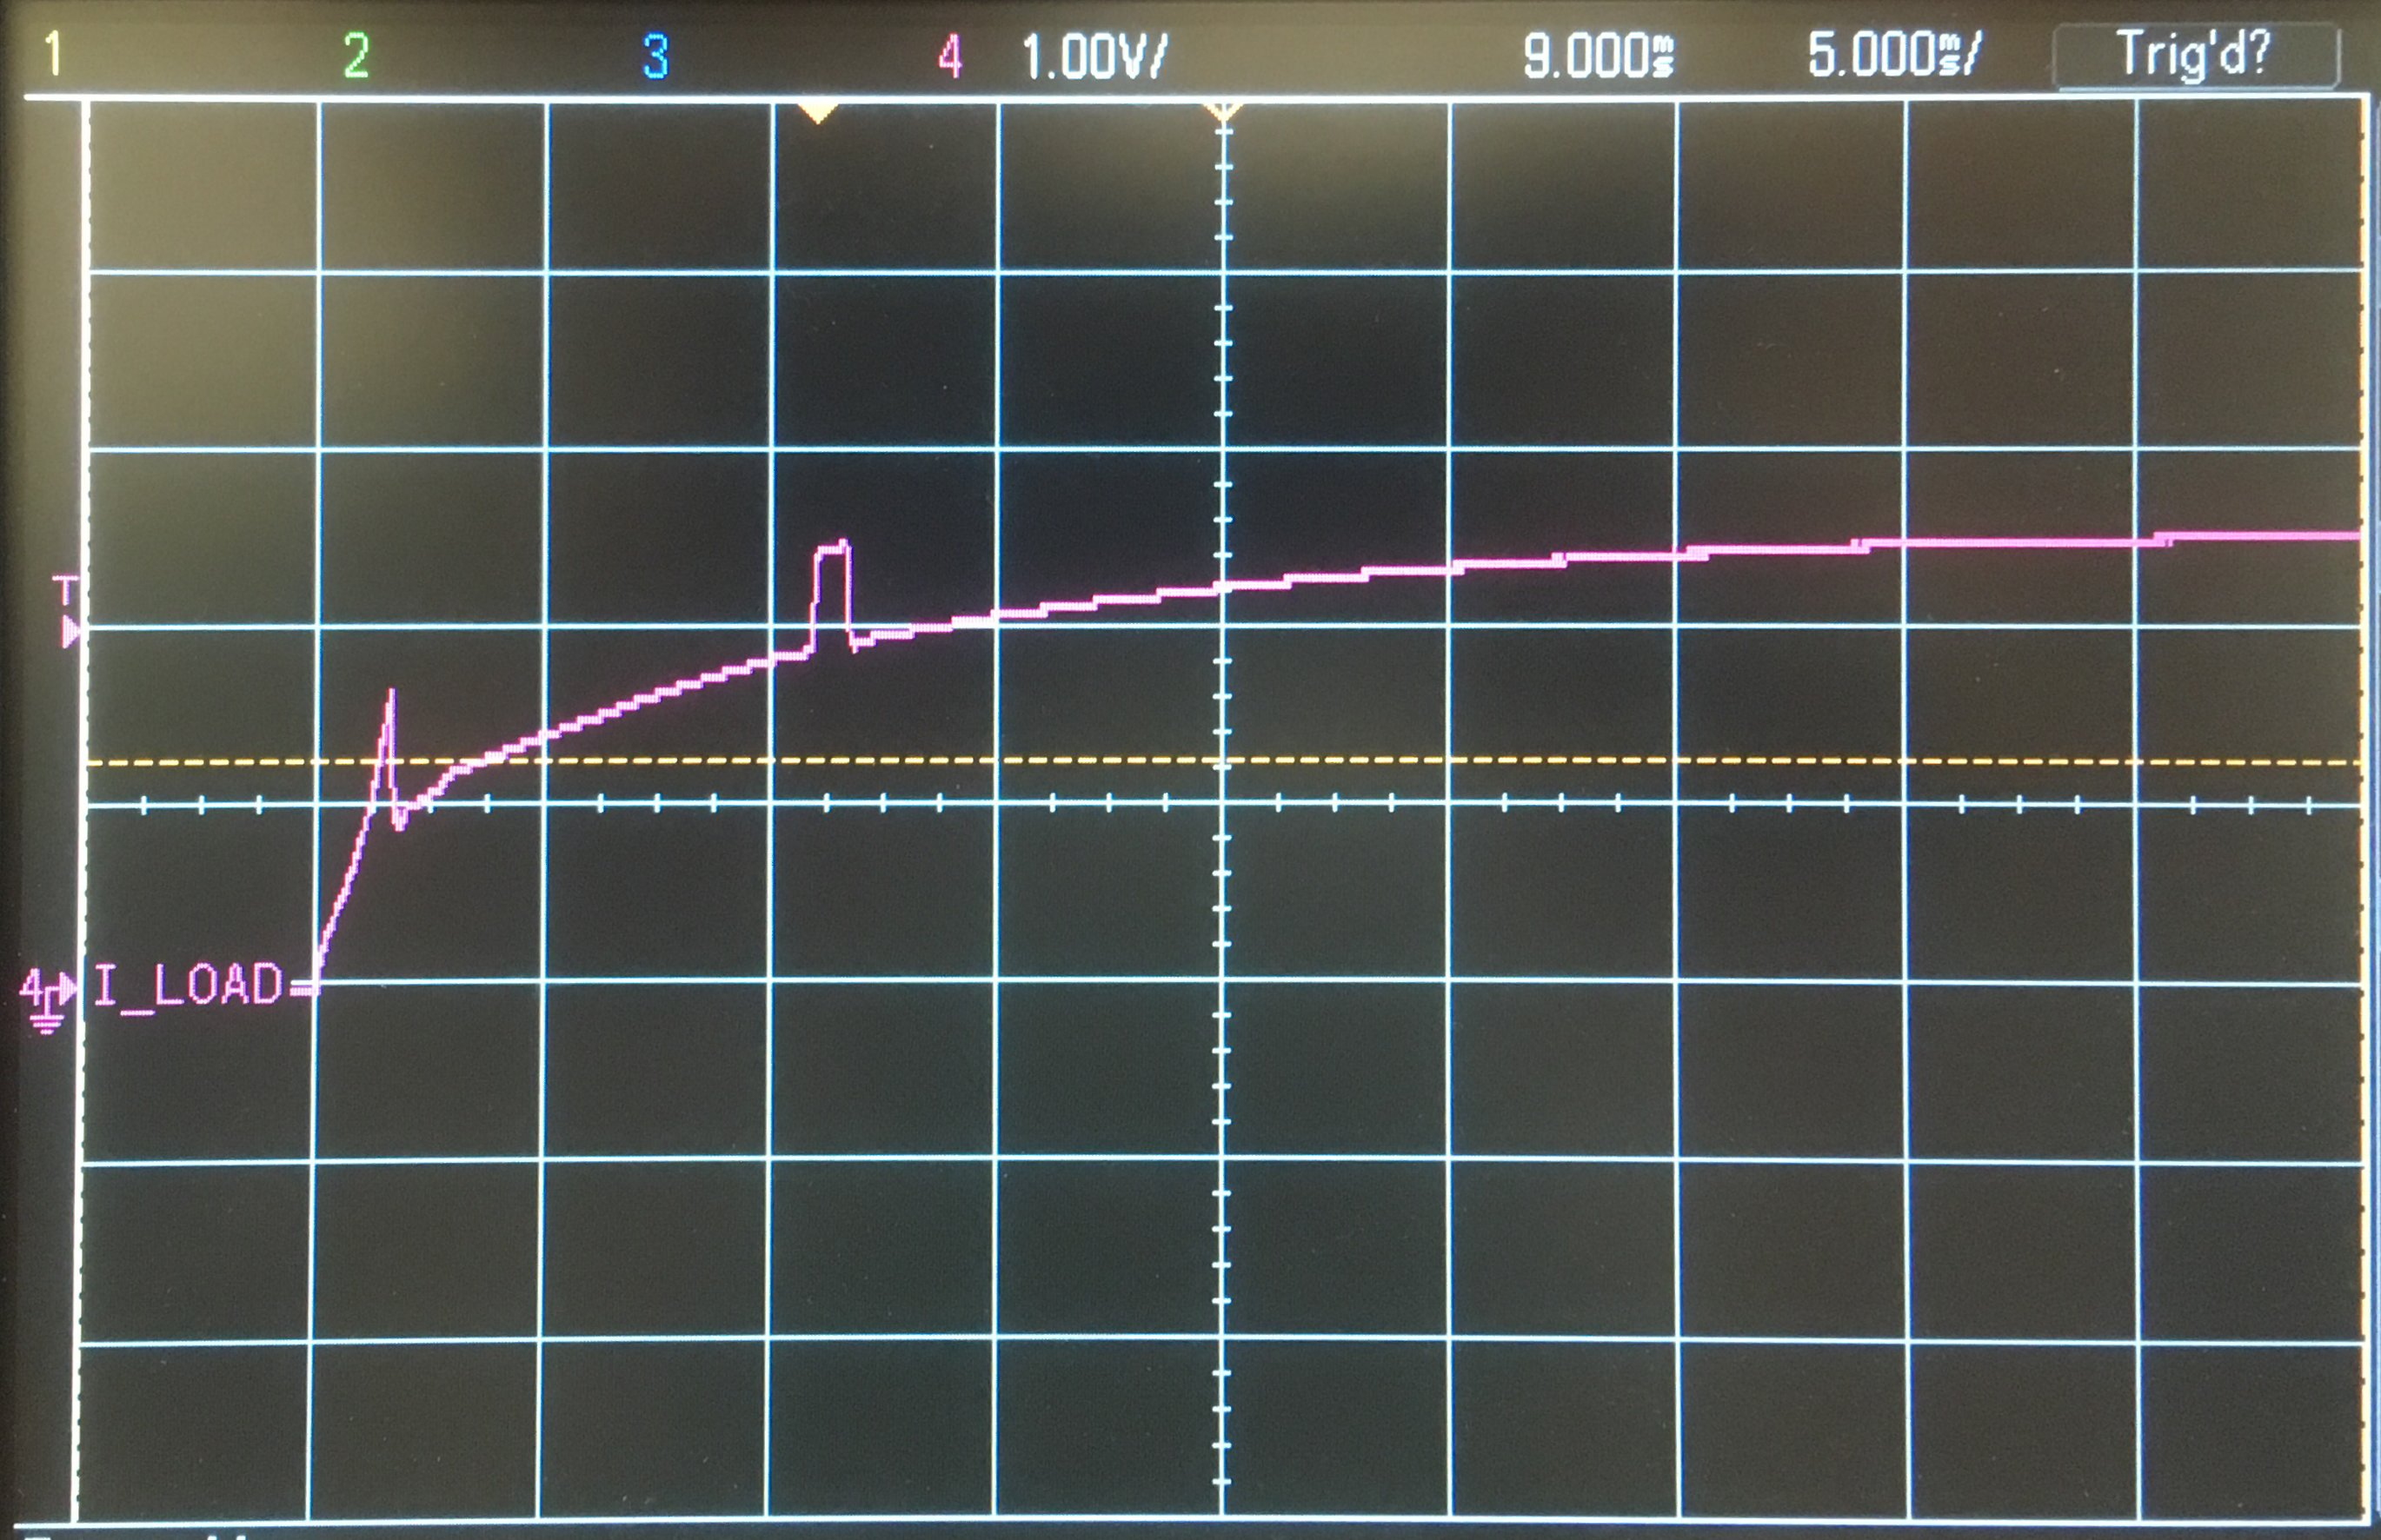
\includegraphics[width=\linewidth]
            {./res/current_transient/power_on-zoom.jpg}
        };
        \draw (zoom1.south west) rectangle (zoom1.north east);
    \end{tikzpicture}
    \caption{}
    \end{subfigure}
    %\begin{tikzpicture}[overlay,boximg]
        %\draw (zoom1) -- (zoombox1);
    %\end{tikzpicture}
    \caption{Power on transient current.}
\end{figure}

\end{document}
